\documentclass[a4paper,10pt]{article}
\usepackage[spanish]{babel}
\usepackage[utf8]{inputenc}
\usepackage{caratula}

\usepackage{amsmath}
\usepackage{amsfonts}
\usepackage[pdftex]{graphicx}
\usepackage{makeidx}
\usepackage{hyperref}
\usepackage{float}
\usepackage{caption}
\usepackage{subcaption}
\usepackage{color}
\usepackage{verbatim}
\usepackage{array}
\usepackage{tabularx}
\usepackage{multicol}
\usepackage{wrapfig}

\usepackage[top=3cm,bottom=2cm,left=2cm,right=2cm]{geometry}

\begin{document}

\materia{Aprendizaje Automático}

\titulo{Homework 4 : Supervised Learning}

\integrante{Martin Miguel}{181/09}{m2.march@gmail.com}

\maketitle
\tableofcontents
\newpage

\section{Introducción}

El presente trabajo presenta una comparativa entre 3 métodos de aprendizaje automático para estimar clasificadores. Se usaron tres aproximaciones distintas al problema de la clasificación: \emph{clasificación estadística} (en particular \textsf{naive bayes}), \emph{árboles de desición} y \emph{aprendizaje basado en instancias}. Para evaluar los métodos se realizaron \emph{cross-validation} con 10 folds sobre el dataset \textsf{adult}\footnote{\url{http://archive.ics.uci.edu/ml/datasets/Adult}}. Además, para hacer una comparación más completa, se ajustaron las configuraciones de los métodos para probar clasificadores más genéricos y más específicos, y todos estos se probaron sobre muestras de datos con ruido variable sobre el valor de la clase objetivo. 

\section{Ejecuciones}

El dataset \textsf{adult} consiste de datos poblacionales obtenidos a partir de censos. Cada instancia dentro del juego de datos hace referencia a una persona censada y posee atributos como la edad, nivel educativo, estado civíl, país de origen, otras métricas económicas y el hecho de si gana o no más de cincuentamil dólares anuales. Este último atributo es el objetivo de la clasificación.

El objetivo del trabajo es lograr comparaciones de las capacidades, fuertes y debilidades de distintos clasificadores bajo 3 ejes de cambio: la técnica utilizada, la cantidad de ruido en la muestra y la especificidad del clasificador. Un clasificador es más específico cuanto más finas son las desiciones que toma para exponer un resultado. Esto es fácil de ver en técnicas como \emph{árboles de desición}\footnote{http://en.wikipedia.org/wiki/Decision\_tree\_learning} o \emph{aprendizaje basado en instancias}. En el primer caso un clasificador es más específico cuanto más profundo es el árbol. En el segundo caso un clasificador es más específico si considera menor cantidad de instancias.
Para \textsf{naive bayes} es más difícil hacer la misma analogía. Se consideró que el clasificador era más específico si utilizaba menor cantidad de atributos.

En el caso particular del \emph{aprendizaje basado en instancias}, el algoritmo utilizado (\textsf{IBk}\footnote{http://en.wikipedia.org/wiki/K-nearest\_neighbor\_algorithm}) permite definir una función para establecer la influencia de las instancias en la clasificación, basado en la distancia a la nueva instancia a clasificar. Uno de los clasificadores no tuvo función de distancia (nomenclado \textsf{no}), por lo que todas las instancias consideradas tenían igual peso en la decisión. Los otros dos clasificadores tuvieron como función de distancias $1/d$ (\textsf{inv}) y $1-d$ (\textsf{min}), con $d$ la distancia entre las intancias. 

Para cada uno de los clasificadores creados (distintas técnicas, distinta especificidad), se evaluó su precisión sobre el mismo juego de datos con distintos niveles de ruido sobre la clasificación. El rudio varió de 0 a 65\%, creciendo en un 1\% cada vez. En un nivel de ruido $x$, $x$\% de las instancias tuvieron cambiada su clase. La precisión se midió como el promedio del porcentaje de clasificaciones correctas para cada uno de los 10 \emph{folds} de la evaluación hecha para el clasificador con el juego de datos ruidoso.

\section{Resultados}

A continuación presentamos cinco gráficos resumiendo los resultados. Agrupamos los clasificadores por técnica y mostramos su precisión sobre nivel de ruido. En el caso de la técnica de clasificación \emph{basada en instancias}, se agruparon además los clasificadores por el tipo de función de distancia utilizada. 

\begin{figure}[h]
\centering
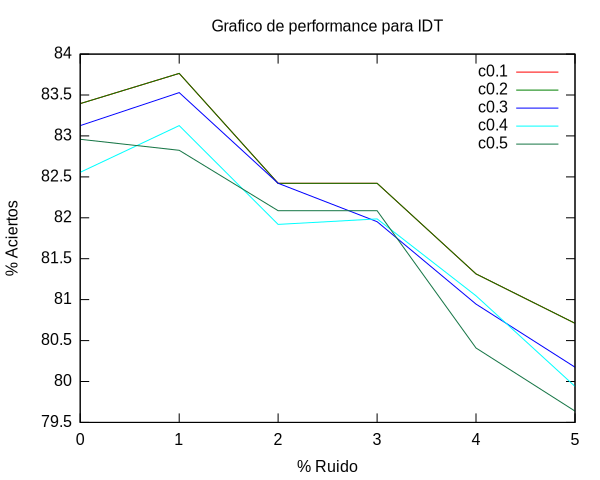
\includegraphics[scale=0.8]{../dats/idt.pdf}
\caption{Gráfico de aciertos de los distintos clasificadores \textsf{IDT} con confianza variable sobre ruido variable.}\label{fig:idt}
\end{figure}

\begin{figure}[h]
\centering
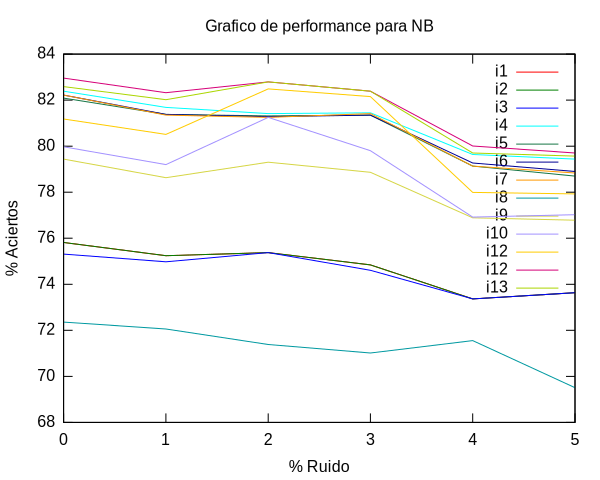
\includegraphics[scale=0.8]{../dats/nb.pdf}
\caption{Gráfico de aciertos de los distintos clasificadores \textsf{NB} con atributos variables sobre ruido variable.}\label{fig:nb}
\end{figure}

\begin{figure}[h]
\centering
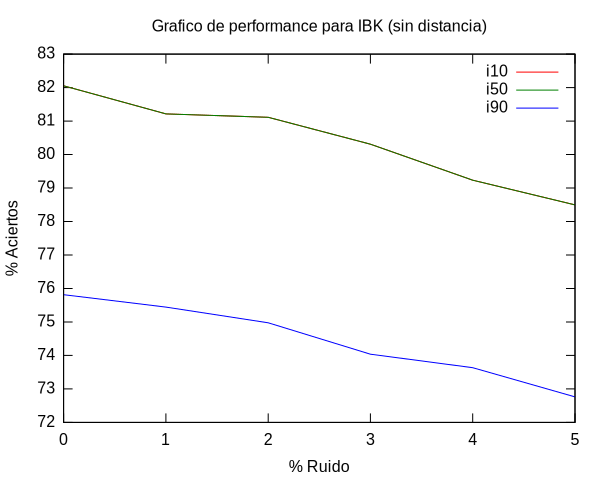
\includegraphics[scale=0.8]{../dats/ibk-no.pdf}
\caption{Gráfico de aciertos de los distintos clasificadores \textsf{IBk} con cantidad variable de instancias sobre ruido variable, sin ponderar las instancias.}\label{fig:ibk-no}
\end{figure}

\begin{figure}[h]
\centering
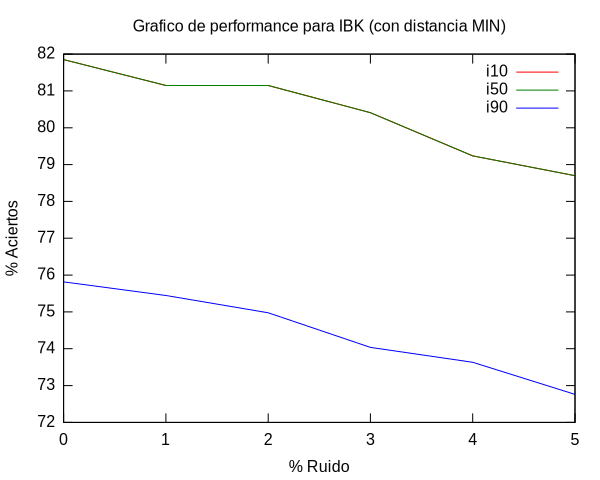
\includegraphics[scale=0.8]{../dats/ibk-min.pdf}
\caption{Gráfico de aciertos de los distintos clasificadores \textsf{IBk} con cantidad variable de instancias sobre ruido variable, con ponderación $1-d$.}\label{fig:ibk-min}
\end{figure}

\begin{figure}[h]
\centering
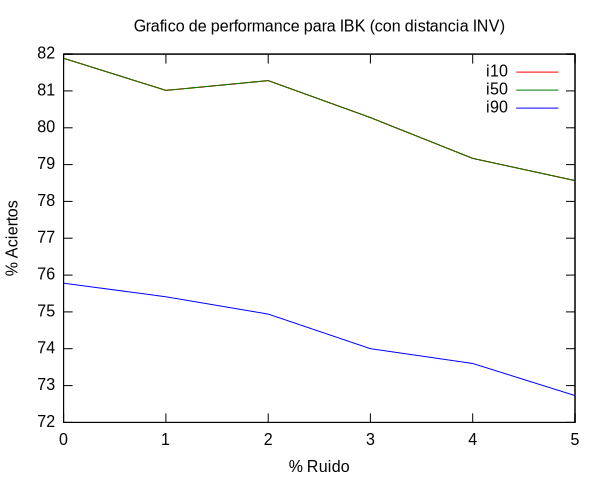
\includegraphics[scale=0.8]{../dats/ibk-inv.pdf}
\caption{Gráfico de aciertos de los distintos clasificadores \textsf{IBk} con cantidad variable de instancias sobre ruido variable, con ponderación $1/d$.}\label{fig:ibk-inv}
\end{figure}

En primer lugar tenemos un comportamiento generalizado para todas las técnicas en todas sus instancias: a mayor ruido peor performance, con el curioso evento donde a partir del 50\% de ruido aumenta el porcentaje de aciertos. En todos los gráficos (exceptuando el de \textsf{naive bayes}), los clasificadores más específicos se notaron con colores más oscuros. E

\section{Conclusiones}



\end{document}

